\documentclass{../tex_import/ETHuebung_english}

\usepackage{../tex_import/exercise_ml}

\input{../tex_import/definitions} %our customized .tex macros

\begin{document}


\makeheader{2, Sept 19, 2024}{Linear Regression and Gradient Descent}

\paragraph{Goals.}
The goal of this week's lab is to
\begin{itemize}
\item Implement grid search, gradient descent and stochastic gradient descent.
\item Learn to debug your implementations.
\item Learn to visualize results.
\item Understand advantages and disadvantages of these algorithms.
\item Study the effect of outliers using MSE and MAE cost functions.
\end{itemize}
~\\

\paragraph{Setup, data and sample code.}
Obtain the folder {\tt labs/ex02} of the course github repository
\begin{center}
\href{https://github.com/epfml/ML\_course/tree/main/labs/ex02}{github.com/epfml/ML\_course}
\end{center}
We will use the dataset {\tt height\_weight\_genders.csv} in this exercise,
and we have provided sample code templates that already contain useful snippets of code
required for this exercise.

You will be working in the notebook {\tt ex02.ipynb} for all exercises of this week, by filling in the corresponding functions. The notebook already provides a lot of template code, as well as code to load the data, and normalize the features, visualize the results.

Additionally, please also take a look at the files {\tt helpers.py} and {\tt plots.py}, and make sure you understand them.


\section{Computing the Cost Function}
In this exercise, we will focus on simple linear regression which takes the following form,
\begin{equation}
y_n \approx f(x_{n1}) = w_0 + w_1 x_{n1}.
\label{eq:f}
\end{equation}
We will use height as the input variable $x_{n1}$ and weight as the output variable $y_n$.
The coefficients $w_0$ and $w_1$ are also called \emph{model parameters}.
We will use a mean-square-error (MSE) function defined as follows,
\begin{equation}
\costfunc \big( w_0, w_1)
= \frac{1}{2N} \sum_{n=1}^N\big(y_n - f(x_{n1}) \big)^2
= \frac{1}{2N} \sum_{n=1}^N\big(y_n - w_0 - w_1 x_{n1} \big)^2.
\label{eq:loss}
\end{equation}
Our goal is to find $w_0^\star$ and $w_1^\star$ that minimize this \emph{cost}.
\newline

Let us start by the array data type in \emph{NumPy}.
We store all the $(y_n,x_{n1})$ pairs in a vector
and a matrix as shown below.
\begin{align}
\yv =
    \left[
    \begin{array}{c}
        y_1\\ y_2\\ \vdots \\ y_N
    \end{array}
    \right] \quad &\quad
\widetilde{\Xm} =
    \left[
    \begin{array}{ccccc}
        1 & x_{11} \\
        1 & x_{21}\\
        \vdots & \vdots\\
        1 & x_{N1}\\
    \end{array}
    \right]
\end{align}

\newpage
\Exercise{1}{
To understand this data format, answer the following warmup questions:
\begin{itemize}
\item What does each \emph{column} of $\Xmt$ represent?
\item What does each \emph{row} of $\Xmt$ represent?
\item Why do we have 1's in $\Xmt$?
\item If we have heights and weights of 3 people, what would be the size of $\yv$ and $\Xmt$?
What would $\Xmt_{32}$ represent?
\item In {\tt helpers.py}, we have already provided code to form arrays for $\yv$ and $\Xmt$.
Have a look at the code, and make sure you understand how they are constructed.
\item Check if the sizes of the variables make sense (use functions {\tt shape}).
\end{itemize}

\begin{enumerate}
\item[a)]
Now we will compute the MSE. Let us introduce the vector notation $\ev = \yv - \Xmt \wv$,
for given model parameters $\wv = [w_0,\, w_1]^\top$.
Show that the MSE can also be rewritten in terms of the vector $\ev$, as
\begin{align}
\costfunc(\wv) = ...
%= \frac{1}{2N} \ev^\top \ev, \textrm{ where } \ev = \yv - \Xmt \wv
\end{align}

\item[b)]
Complete the implementation of the notebook function {\tt compute\_loss(y, tx, w)}.
You can start by setting $\wv = [1, 2]^\top$, and test your function.
\end{enumerate}
}

\section{Grid Search}
Now we are ready to implement our first optimization algorithm: Grid Search. Refer to the lecture notes for a description of the algorithm.


\Exercise{2}{
\begin{enumerate}
\item[a)]
Fill in the notebook function {\tt grid\_search(y, tx, w0, w1)} to implement grid search.
You will have to write one for-loop per dimension, and compute the cost function
for each setting of $w_0$ and $w_1$.
Once you have all values of cost function stored in the variable {\tt loss},
the code finds an approximate minimum (as discussed in the class).

The code should print the obtained minimum value of the cost function
along with the found $w_0^\star$ and $w_1^\star$. It should also show a contour plot
and the plot of the fit, as shown in Figure~\ref{fig:grid_search}.

\begin{figure}[!htp]
\centering
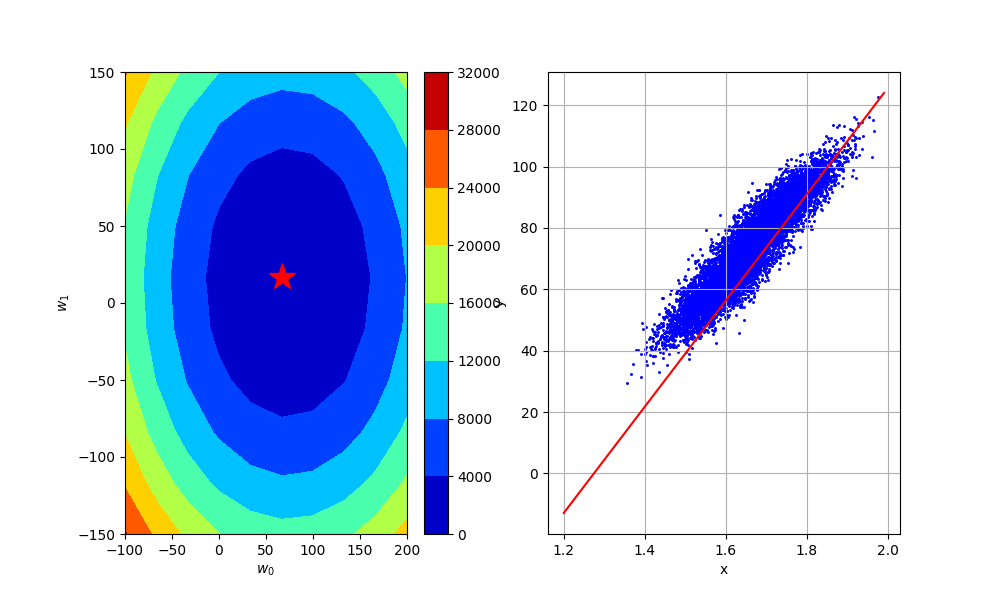
\includegraphics[width=11cm, height=7cm]{solution/grid_plot.png}\vspace{-1em}
\caption{Grid Search Visualization}
\label{fig:grid_search}
\end{figure}

\item[b)]
Does this look like a good estimate? Why not?
What is the problem? Why is the MSE plot not smooth?

Repeat the above exercise by changing the grid spacing to 10 instead of 50.
Compare the new fit to the old one.

\item[c)]
Discuss with your peers:
\begin{itemize}
\item To obtain an accurate fit, do you need a coarse grid or a fine grid?
\item Try different values of grid spacing. What do you observe?
\item How does increasing the number of values affect the computational cost? How
fast or slow does your code run?
\end{itemize}

\end{enumerate}
}

\section{Gradient Descent}
In the lecture, we derived the following expressions for the gradient (the vector of partial derivatives) of the MSE for linear regression,
\begin{align}
\frac{\partial \costfunc (w_0, w_1)}{\partial w_0}
    &= -\frac{1}{N} \sum_{n=1}^{N} \big(y_n - w_0 - w_1 x_{n1}\big)
        = - \frac{1}{N} \sum_{n=1}^N e_n \\
\frac{\partial \costfunc (w_0, w_1)}{\partial w_1}
    &= -\frac{1}{N} \sum_{i=1}^{N}  \big(y_n - w_0 - w_1 x_{n1} \big) x_{n1}
        = - \frac{1}{N} \sum_{n=1}^N e_n x_{n1}
\end{align}
Denoting the gradient by $\nabla \costfunc(\wv)$, we can write these
operations in vector form as follows,
\begin{align}
\nabla \costfunc(\wv)
    :=
    \left[
        \begin{array}{c}
            \frac{\partial \costfunc (w_0, w_1)}{\partial w_0}
            \frac{\partial \costfunc (w_0, w_1)}{\partial w_1}
    \end{array}
    \right]
    = -\frac{1}{N}
    \left[
        \begin{array}{c}
            \sum_{n=1}^N e_n \\ \sum_{n=1}^N e_n x_{n1}
        \end{array}
        \right]
    = -\frac{1}{N} \Xmt^\top \ev
\label{eq:gradients}
\end{align}


\Exercise{3}{
\begin{enumerate}
\item[a)]
Now implement a function that computes the gradients.
Implement the notebook function {\tt compute\_gradient(y, tx, w)}
using Equation~\eqref{eq:gradients}.
Verify that the function returns the right values.
First, manually compute the gradients for hand-picked values of $\yv$, $\Xmt$,
and $\wv$ and compare them to the output of {\tt compute\_gradient}.

\item[b)]
Once you make sure that your gradient code is correct, get some intuition about
the gradient values:

Compute the gradients for
\begin{itemize}
\item $w_0=100$ and $w_1=20$
\item $w_0=50$ and $w_1=10$
\end{itemize}
What do the values of these gradients tell us? For example, think about the norm
of this vector. In which case are they bigger? What does that mean?

\emph{Hint:} Imagine a quadratic function and estimate its gradient near
its minimum and far from it.

\emph{Hint 2:} As we know from the lecture notes, the update rule for gradient descent at step
$t$ is
\begin{equation}
\wv^{(t+1)} = \wv^{(t)} - \gamma \, \nabla \costfunc(\wv^{(t)})
\end{equation}
where $\gamma>0$ is the step size, and $\nabla \costfunc \in \R^2$ is the gradient vector.

\item[c)]
Fill in the notebook function {\tt gradient\_descent(y, tx, initial\_w, ...)}.
Run the code and visualize the iterations.
Also, look at the printed messages that show $\costfunc$ and
values of $w_0^{(t)}$ and $w_1^{(t)}$.
Take a detailed look at these plots,
\begin{itemize}
\item Is the cost being minimized?
\item Is the algorithm converging? What can be said about the convergence speed?
\item How good are the final values of $w_1$ and $w_0$ found?
\end{itemize}


\item[d)]
Now let's experiment with the value of the step size and initialization parameters
and see how they influences the convergence.
In theory, gradient descent converges to the optimum on convex functions,
when the value of the step size is chosen appropriately.

\begin{itemize}
\item Try the following values of step size: 0.001, 0.01, 0.5, 1, 2, 2.5.
What do you observe? Did the procedure converge?

\item Try different initializations with fixed step size $\gamma=0.1$, for instance:
    \begin{itemize}
        \item $w_0=0$, $w_1=0$
        \item $w_0=100$, $w_1=10$
        \item $w_0=-1000$, $w_1=1000$
    \end{itemize}
    What do you observe? Did the procedure converge?
\end{itemize}

\end{enumerate}
}

\section{Stochastic Gradient Descent}
\Exercise{4}{
Let us implement stochastic gradient descent. Recall from the lecture notes that the update rule for stochastic gradient descent on an objective function $\costfunc(\wv) = \tfrac1N\sum_{n=1}^N \costfunc_n(\wv)$
at step $t$ is
\begin{equation}
\wv^{(t+1)} = \wv^{(t)} - \gamma \, \nabla \costfunc_n(\wv^{(t)}) \ .
\end{equation}

HINT: You can use the function {\tt batch\_iter()} in the file of {\tt helpers.py}
to generate mini-batch data for stochastic gradient descent.
%TODO: the small set (usually size 1) over which we compute the stochastic gradient should be called mini-batch always (TODO change in the code also). Also, to avoid confusion the alternative is to just use size one always. would be easier for the students to understand at this early stage.

What differences do you observe between the gradient descent and stochastic gradient descent procedures?
}

\section{Effect of Outliers and MAE Cost Function}
In the course we talked about \emph{outliers}.
Outliers might occur due to measurement errors.
For example, in the weight/height data, a coding mistake could introduce points
whose weight is measured in pounds rather than kilograms.

Such outlier points may have a strong influence on model parameters.
For example, MSE (the one you implemented above) is known to be sensitive to outliers,
as discussed in the class.

\Exercise{5}{
Let's simulate the presence of two outliers, and their effect on linear
regression under MSE cost function,
\begin{itemize}
\item Reload the data through function {\tt load\_data()} by setting {\tt sub\_sample=True}
to keep only a few data examples.
\item Plot the data. You should get a cloud of points similar, but less dense,
than what you saw before with the whole dataset.
\item As before, find the values of $w_0,w_1$ to fit a linear model (using MSE cost function), and plot
the resulting $f$ together with the data points.
\item Now we will add two outliers points simulating the mistake that we entered
the weights in pounds instead of kilograms.
For example, you can achieve this by setting {\tt add\_outlier=True} in {\tt load\_data()}. Feel free to add more outlier points.
\item Fit the model again to the augmented dataset with the outliers. Does it look like a good fit?
\end{itemize}
}

\newpage
One way to deal with outliers is to use a more \emph{robust} cost function,
such as the Mean Absolute Error (MAE), as discussed in the class.

\section{Subgradient Descent}

\Exercise{6}{
Modify the function {\tt compute\_loss(y, tx, w)} for the Mean Absolute Error cost function.
\newline

Unfortunately, you cannot directly use gradient descent, since the MAE function is non-differentiable at several points.

\begin{enumerate}
\item[a)]
Compute a subgradient of the MAE cost function, for every given vector $\wv$. 

\par\emph{Hint: Use the chain rule to compute the subgradient of the absolute value function. 
For a function $\mathcal{L}(\wv) := h(q(\wv))$ with $q$ differentiable, the subgradient can be computed using $\partial \mathcal{L} (\wv) = \partial h(q(\wv)) \cdot \nabla q(\wv)$, where each $\partial..$ denotes the set of all subgradient vectors.}

\item[b)]
Implement subgradient descent for the MAE cost function.

To do so, write a new function {\tt compute\_subgradient(y, tx, w)} for the new MAE objective which returns a subgradient if the given $\wv$ turns out to be a non-differentiable point.

%Use the grid search script that you wrote to fit a model to the augmented data
%that contains the outliers.
Plot the resulting model $f$ together with the two curves obtained in the previous exercise.
\begin{itemize}
\item Is the fit using MAE \emph{better} than the one using MSE?
\item Did your optimization algorithm ever encounter a non-differentiable point?
%\item You can see in the contour plot that the cost function is not strictly convex.
%How would this affect the optimization? Think about it. %TODO: too hard, too unspecific
% \item Bonus question: try Huber loss using gradient descent.
\end{itemize}

\item[c)]
Implement stochastic subgradient descent (SGD) for the MAE cost function.

How is the picture different when you compare the two algorithm variants on MAE, compared to what you have observed on MSE?

\end{enumerate}
}

\section*{Wrap-Up}
After you have finished the implementation of the above exercises the notebook {\tt ex02.ipynb}, you can wrap up by copying your code to separate {\tt .py} files for later re-use. For example, you'll be re-using your code from this week later on, for example for Project 1 and some of the subsequent labs.

We have provided template files for this, namely\\
{\tt cost.py, grid\_search.py, gradient\_descent.py} and {\tt stochastic\_gradient\_descent.py},


\end{document}
